\newpage
\section{Graphical models}
As the number of variables we wish to model increases the number of different models increases faster than exponentially. A common technique to get a handle on the dependencies of many real-world variables is to organize them into connected structures the components of which are simple and easily interpretable. This allows us to construct hierarchies, a powerful method for synthesizing knowledge.

Representing variables with the nodes and dependencies with the edges of a graph is a powerful method to gain a bird's eye view of the model and reason about statistical dependencies between the variables under different fixed conditions. This section introduces elements of a graphical representation technique using directed, acyclic graphs. (Other methods are undirected graphs and factor graphs.)

\subsection{Elements}
\begin{itemize}
	\item A {\bf directed connection} from variable $x$, to variable $y$, indicates that we intend to describe their joint distribution using the conditional probability $P(y\;|\;x)$, i.e. $P(x, y) = P(y\;|\;x) P(x)$. The graphical representation of this is
	\begin{figure}[h]
	\centering
		\includegraphics[height=3.4mm]{./figs/04-xy.pdf} 
	\end{figure}

	\item A {\bf chain} of connections, which is formed by two directed connections, one from $x$ to $z$ and another from $z$ to $y$, indicates that we intend to describe the joint as $P(x, y, z) = P(y\;|\;z) P(z\;|\;x) P(x)$. This is represented by a the following graph.
	\begin{figure}[h]
	\centering
		\includegraphics[height=3.4mm]{./figs/04-xzy.pdf} 
	\end{figure}

	Note: This graph represents a restriction to the set of distributions for the joint, because the variable $z$ separates $x$ and $y$, indicating that $x$ and $y$ become independent once we fix the value of $z$ (to any value), i.e. $P(x,y\;|\;z) = P(x\;|\;z) P(y\;|\;z)$. This, we write as $y \independent x \;|\;z$. On the other hand, if $z$ is unknown, $x$ and $y$ may be dependent, which we write as $y \not\independent x\; | \; \emptyset$. The $z$ variable in the middle in such situations is called the ``mediator'' between $x$ and $y$.

	\item A {\bf fork} is formed when two connections originate from one variable $x$ and connect to two different variables $y_1$ and $y_2$, indicating that we intend to describe their joint as $P(x, y_1, y_2) = P(y_1\;|\;x) P(y_2\;|\;x) P(x)$. This is represented by a the following graph.
	\begin{figure}[h]
	\centering
		\includegraphics[height=12mm]{./figs/04-xy1y2.pdf} 
	\end{figure}

	Note: This dependency structure implied by this graph (on its own) is identical to the dependency structure of the chain, i.e. $y_1 \independent y_2 \;|\;x$, and $y_1 \not\independent y_2\; | \; \emptyset$, but the interpretation is different. Variables $x$ is interpreted as a ``common cause'' for $y_1$ and $y_2$.

	\item The {\bf collider}, which is formed by directed connections from two variables $x_1$ and $x_2$ to one variable $y$, is the most interesting graphical element. It indicates that we believe that $x_1$ and $x_2$ are independent variables, i.e. the we expect to write the joint as $P(x_1, x_2, y) = P(y\;|\;x_1, x_2) P(x_1) P(x_2)$. This is represented by a the following graph.
	\begin{figure}[h!]
	\centering
		\includegraphics[height=12mm]{./figs/04-x1x2y.pdf} 
	\end{figure}

	Note: By definition, this dependency structure implies $x_1 \independent x_2\;|\;\emptyset$, however the same does not hold if the value of $y$ is fixed, $x_1 \not\independent x_2\;|\;y$. This effect is called ``explaining away''.
	
\end{itemize}

\subsection{General rules}

\no {\bf Converting between graph and formula}\\ 
The general rules for converting between a graphical representation and the formula of the joint distribution are the following
\begin{itemize}
	\item Each variable $x$ (node of the graph) contributes a factor $P(x\;|\ldots)$ to the formula. The only question is what should go in place of $\ldots$ in the condition part.

	\item If the node has no incoming edges, the condition part should be left empty, i.e. the factor is $P(x\;|\;\emptyset) = P(x)$.

	\item If the node has incoming connections, the variables from which the connections originate (``parents'') should be listed in the condition part, i.e. the factor is $P(x\;|\;\text{parents of }x)$.
\end{itemize}


\no {\bf d-separation}\\
Two variables are said to be ``d-separated'' if their independence (under specific conditions) is implied by the graph structure. For the general case of trying to determine independence between $x$ and $y$ under the condition of keeping variables $z_1, z_2, \ldots z_c$ fixed, the steps are the following.
\begin{enumerate}
	\item List all possible paths between $x$ and $y$ through the graph disregarding the directions of the connections (i.e. moving in the opposite direction of the connections is also allowed). Each node is allowed to be visited at most once in every path.

	\item For each node on each path, mark the way it is traversed with respect to the direction of the connections: mediator ($\leftarrow\leftarrow$ or $\rightarrow\rightarrow$), fork ($\leftarrow\rightarrow$) or collider ($\rightarrow\leftarrow$). (Note: It is possible for a node with three or more connections to be traversed differently by different paths.)

	\item Disregard all paths of which any of the mediator or fork nodes is among the $\{z_1, z_2, \ldots z_c\}$ variables, on which we are conditioning. These paths are ``blocked''.

	\item On the remaining paths, investigate the colliders. Going against our intuition, a collider blocks the path if {\bf neither} itself {\bf nor} any of its descendents is among $\{z_1, z_2, \ldots z_c\}$. (E.g. if we do not condition on any variable, then all paths that traverse at least one node in collider fashion are blocked.) Disregard these paths.

	\item If all paths are blocked, in one way or another, $x$ and $y$ are conditionally independent, conditioned on the variables $z_1, z_2, \ldots z_c$, which we write as $x \independent y\;|\; z_1, z_2, \ldots z_c$.
\end{enumerate}

\no {\bf Examples}
\begin{itemize}
	\item $P(a, b, c, d, e) = P(a)P(d) P(b\;|\;a,d) P(c\;|\;b) P(e\;|\;c) P(f\;|\;c)$ is represented by 

	\begin{figure}[h!]
	\centering
		\includegraphics[height=15mm]{./figs/04-abcdef.pdf} 
	\end{figure}
	Some examples of d-separation are $e \independent f \;|\; c$,\quad $e \independent a \;|\; b$ and $a \independent d \;|\;\emptyset$, (but $a \not\independent d \;|\;b$ and $a \not\independent d \;|\;f$).

	\item $P(a, b, c, d, e, f) = P(a) P(c\;|\;a) P(b\;|\;a) P(f\;|\;c) P(d\;|\;b, c) P(e\;|\;d)$ is represented by

	\begin{figure}[h!]
	\centering
		\includegraphics[height=20mm]{./figs/04-abcdef2.pdf} 
	\end{figure}
	Some examples of d-separation are $b \independent f \;|\; a$ and  $b \independent f \;|\; a,c,e$ (but $b \not\independent f \;|\; a,d$ and $b \not\independent f \;|\; a,e$).
\end{itemize}

\newpage
\subsection{Real-life examples}
\begin{itemize}
	\item Fire causes Smoke, Smoke causes Alarm to set off, but given Smoke, there's no correlation between Fire and Alarm, i.e. $\text{Fire}\;\independent\;\text{Alarm}\;|\;\text{Smoke}$. This is represented by a chain
	\begin{figure}[h!]
	\centering
		\includegraphics[height=2.5mm]{./figs/04-fire-smoke-alarm.pdf} 
	\end{figure}

	\item Both rain and the Sprinkler can cause the formation of a Puddle, they are however independent (until we observe the Puddle), i.e. $\text{Rain}\;\independent\;\text{Sprinkler}\;|\;\emptyset$. This is represented by a collider
	\begin{figure}[h!]
	\centering
		\includegraphics[height=12.5mm]{./figs/04-rain-puddle-sprinkler.pdf} 
	\end{figure}

	\item Heat causes both Ice Cream sales and Crime to increase, but once we know there was a heatwave, they become independent, i.e. $\text{Crime}\;\independent\;\text{Ice Cream}\;|\;\text{Heat}$. This is represented by a fork
	\begin{figure}[h!]
	\centering
		\includegraphics[height=10.5mm]{./figs/04-heat-icecream-crime.pdf} 
	\end{figure}

	\item Education affects Political View, which affects both Party membership and Voting behavior. This can be represented as
	\begin{figure}[h!]
	\centering
		\includegraphics[height=14.4mm]{./figs/04-education-vote.pdf} 
	\end{figure}

	\item Education and Experience both affect Salary, but Education also affects Experience. This can be represented as
	\begin{figure}[h!]
	\centering
		\includegraphics[height=18mm]{./figs/04-education-salary.pdf} 
	\end{figure}
\end{itemize}

\subsection{Plate notation}
When a series of variables are connected to the rest of the graph in identical fashion, we simplify our notation by placing a representative of the variable series inside a box (``on a plate'') in place of the series, and label the box with the length of the series.
\begin{figure}[h!]
\centering
	\includegraphics[height=30mm]{./figs/04-plate-notation.pdf}
\end{figure}

\newpage
\subsection{Hierarchical models}

\no {\bf Beta-Binomial model}
\begin{itemize}
	\item Data: $D = \{(k_i, n_i)\}_{i=1}^N$, where $k_i$(successes) $\in\{0, 1, \ldots n_i\}$, and $n_i$(attempts) $\in \mathds{N}$

	\item Model: 
		\begin{itemize}
			\item level 1: the parameters, $p = \{p_i\}_{i=1}^N$, where $p_i \in [0,1]$, define $P(k_i\;|\;n_i, p_i) = \text{Binomial}(k_i\;|\;n_i, p_i)$
			\item level 2: the parameters, $\alpha, \beta$ (both $>0$), define $P(p_i\;|\;\alpha, \beta) = \text{Beta}(p_i\;|\;\alpha, \beta)$.
		\end{itemize}
		This hierarchy can be represented as
		\begin{figure}[h!]
		\centering
			\includegraphics[height=26mm]{./figs/04-BetaBinomial.pdf}
		\end{figure}

	\item Joint likelihood:
	\be
		P(D, p\;|\;\alpha,\beta) = \prod_{i=1}^N\Big[\text{Binom}(k_i\;|\;n_i, p_i) \;\text{Beta}(p_i\;|\;\alpha, \beta)\Big]
	\ee

	\item Marginal likelihood:
	\ba
		P(D\;|\;\alpha, \beta) &=& \prod_{i=1}^N\left[\int\!dp_i\,\text{Binom}(k_i\;|\;n_i, p_i) \;\text{Beta}(p_i\;|\;\alpha, \beta)\right] = \prod_{i=1}^N\Big[\text{Beta-Binom}(k_i\;|\;n_i, \alpha, \beta)\Big]
		\\
		\text{where}&&
		\text{Beta-Binom}(k\;|\;n, \alpha, \beta) = \frac{\Gamma(n+1)\Gamma(\alpha + \beta)}{\Gamma(n + \alpha + \beta)} \frac{\Gamma(k+\alpha)}{\Gamma(k+1) \Gamma(\alpha)} \frac{\Gamma(n - k + \beta)}{\Gamma(n-k + 1) \Gamma(\beta)}
	\ea
\end{itemize}

\no {\bf Gamma-Poisson model} (aka. Negative Binomial model)
\begin{itemize}
	\item Data: $D = \{k_i\}_{i=1}^N$, where $k_i$(events) $\in \mathds{N}$.
	\item Model: 
	\begin{itemize}
		\item level 1: the parameters $\lambda = \{\lambda_i\}_{i=1}^N$, where $\lambda_i$ > 0, define $P(k_i\;|\;\lambda) = \text{Poisson}(k_i\;|\;\lambda_i)$
		\item level 2: the parameters $\alpha, \beta$ (both $>0$), define $P(\lambda_i\;|\; \alpha, \beta) = \text{Gamma}(\lambda_i\;|\;\alpha, \beta)$.
	\end{itemize}
	This hierarchy can be represented as 
	\begin{figure}[h!]
		\centering
			\includegraphics[height=26mm]{./figs/04-GammaPoisson.pdf}
		\end{figure}
	\item Joint likelihood:
	\be
		P(D, \lambda\;|\;\alpha, \beta) = \prod_{i=1}^N\Big[\text{Poisson}(k_i\;|\;\lambda_i) \;\text{Gamma}(\lambda_i\;|\;\alpha, \beta)\Big]
	\ee

	\item Marginal likelihood:
	\ba
		P(D\;|\;\alpha, \beta) &=& \prod_{i=1}^N\left[\int\!d\lambda_i\,\text{Poisson}(k_i\;|\;\lambda_i) \;\text{Gamma}(\lambda_i\;|\;\alpha, \beta)\right] = \prod_{i=1}^N\Big[\text{Gamma-Poisson}(k_i\;|\;\alpha, \beta)\Big]
		\\
		\text{where} && \text{Gamma-Poisson}(k\;|\;\alpha, \beta) = \frac{\Gamma(k + \alpha)}{\Gamma(k+1)\Gamma(\alpha)} \left(\frac{1}{\beta + 1}\right)^k \left(\frac{\beta}{\beta + 1}\right)^\alpha = 
		\\
		&=&
		\text{NegativeBinom}(k\;|\;r, p) = {k + r -1 \choose k} p^k (1-p)^r,\quad \text{with }r = \alpha, \; p = \frac{1}{\beta + 1}
	\ea
\end{itemize}

\no {\bf Dirichlet-Multinomial model}
\begin{itemize}
	\item Data: $D = \{k_i\in\mathds{N}^M\}_{i=1}^N = \{(k_{i,1}, k_{i,2}, \ldots k_{i,M})\}_{i=1}^N$, where $k_{i,j}$(number of outcome $j$) $\in \mathds{N}$
	\item Model:
	\begin{itemize}
		\item level 1: the parameters $p = \{p_i \in \mathds{R}^{M}\}_{i=1}^N = \{(p_{i,1}, p_{i,2},\ldots p_{i,M})\}_{i=1}^N$, where $p_{i,j}$(probability of outcome $j$ in sample $i$) $>0$, and $\sum_{j=1}^M p_{i,j} = 1,\;\forall i$, define $P(k_i\;|\;p_i) = \text{Multinomial}(k_i\;|\;k_{i,\text{tot}},p_i)$, where $k_{i,\text{tot}} = \sum_{j=1}^M k_{i,j}$
		\item level 2: the parameters $\alpha = (\alpha_1, \alpha_2, \ldots \alpha_M)$, where each $\alpha_j > 0$, define $P(p_i\;|\; \alpha)= \text{Dirichlet}(p_i\;|\;\alpha)$
	\end{itemize}
	This hierarchy can be represented as 
	\begin{figure}[h!]
		\centering
			\includegraphics[height=26mm]{./figs/04-DirichletMultinomial.pdf}
		\end{figure}
	\item Joint likelihood:
	\be
		P(D\;p|\;\alpha) = \prod_{i=1}^N\Big[ \text{Multinomial}(k_i\;|\;k_{i,\text{tot}}, p_i)\;\text{Dirichlet}(p_i\;|\alpha) \Big]
	\ee
	\item Marginal likelihood:
	\ba
		P(D\;|\;\alpha) &=& \prod_{i=1}^N\left[\int\!dp_i\, \text{Multinomial}(k_i\;|\;k_{i,\text{tot}}, p_i)\;\text{Dirichlet}(p_i\;|\alpha) \right] = \prod_{i=1}^N\Big[\text{Dirichlet-Multinomial}(k_i\;|\;k_{i,\text{tot}}, \alpha)\Big]
		\\
		\text{where} && \text{Dirichlet-Multinomial}(k\;|\;k_\text{tot}, \{\alpha_j\}_{j=1}^M) = \frac{\Gamma(k_\text{tot}+1)\Gamma(\alpha_\text{tot})}{\Gamma(k_\text{tot} + \alpha_\text{tot})} \prod_{j=1}^M \frac{\Gamma(k_j + \alpha_j)}{\Gamma(k_j + 1)\Gamma(\alpha_j)},
		\\
		&&\text{where }\quad \alpha_\text{tot} = \sum_{j=1}^M \alpha_j
	\ea
\end{itemize}

\newpage
\no {\bf Random Effect Model}
\begin{itemize}
	\item Data: $D = \{x_g\}_{g=1}^G = \{(x_{g,1}, x_{g,2},\ldots x_{g, N_g})\}_{g=1}^G$, where $x_{g,i} \in \mathds{R}$ is measurement $i$ in group $g$, and groups can be of different sizes $N_g$.
	\item Model:
	\begin{itemize}
		\item level 1: The parameters $\mu = \{\mu_g\}_{g=1}^G$ and $\sigma^2$ define $P(x_{g,i}\;|\;\mu_g, \sigma) = \text{Normal}(x_{g,i}\;|\;\mu_g, \sigma^2)$
		\item level 2: The parameter $\sigma_0^2$ define $P(\mu_g\;|\;\mu_0,\sigma_0) = \text{Normal}(\mu_g\;|\;\mu_0, \sigma_0^2)$
	\end{itemize}
	This hierarchy can be represented as  
	\begin{figure}[h]
		\centering
			\includegraphics[height=26mm]{./figs/04-anova.pdf}
	\end{figure}
	\item Joint likelihood:
	\be
		P(D, \mu\;|\; \mu_0, \sigma_0, \sigma) = \prod_{g=1}^G\left[\text{Normal}(\mu_g\;|\;\mu_0, \sigma_0^2) \times \prod_{i=1}^{N_g}\text{Normal}(x_{g,i}\;|\;\mu_g, \sigma^2)\right]
	\ee
	\item Marginal likelihood:
	\ba
		P(D\;|\;\mu_0, \sigma_0, \sigma) 
		&=& 
		\prod_{g=1}^G\intop_{-\infty}^{+\infty}\!d\mu_g\,\left[\text{Normal}(\mu_g\;|\;\mu_0, \sigma_0^2) \times \prod_{i=1}^{N_g}\text{Normal}(x_{g,i}\;|\;\mu_g, \sigma^2)\right] 
		\\
		&=&
		(2\pi \sigma_0^2)^{-\frac{G}{2}} \prod_{g=1}^G \left[\frac{1}{\sqrt{\xi + N_g}}(2\pi\sigma^2)^{-\frac{N_g-1}{2}}\exp\left(-\frac{N_g}{2\sigma^2}\left[\frac{\xi}{\xi + N_g}(\mu_g - m_g)^2 + s_g^2\right]\right)\right]
		\\
		\text{where}&& \xi = \frac{\sigma^2}{\sigma_0^2},\qquad m_g = \frac{1}{N_g}\sum_{i=1}^{N_g} x_{g,i}, \qquad s_g^2 = \frac{1}{N_g}\sum_{i=1}^{N_g} x_{g,i}^2 - m_g^2
	\ea

\end{itemize}

\newpage
\subsection{Example: Beta-Binomial}
Life-time performance 10 different boxers are collected. Wins ($k_i$) and losses ($n_i - k_i$) are tallied, and the observed win rate $p_{i,\text{obs}} = k_i / n_i$ is calculated. This is shown below
\begin{figure}[h]
\centering
	\includegraphics[width=0.7\textwidth]{./figs/04-betabinom-data.pdf}
\end{figure}

We would like to determine the win rate of an ``typical boxer'', i.e. the distribution of the win rate $p$. While the observed values $p_\text{obs}$ are good estimates of the individual win rates, 5 boxers played less than 30 matches, while 5 played more than 40, which means the second group provides more information, and their observed win rates need to be taken with more certainty. The Beta-Binomial hierarchical model accounts for this inhomogeneity.
\begin{itemize}
	\item Data: $\{n_i\} = [24, 23, 30, 21, 25, 53, 41, 52, 64, 57]$, $\{k_i\} = [ 10, 13,  9, 10,  9, 51, 28, 37, 59, 45]$, with $N = 10$.
	\item Parameters: $\alpha, \beta > 0$
	\item Model:
	\ba
		&& \log P(D\;|\;\alpha, \beta) = \sum_{i=1}^N \log \Big(\text{Beta-Binom}(k_i\;|\;n_i, \alpha, \beta)\Big)
		\\
		&\text{where}&
		\log\Big(\text{Beta-Binom}(k\;|\;n, \alpha, \beta)\Big) = -f(n, \alpha+\beta) + f(k, \alpha) + f(n-k, \beta),
		\\
		&\text{where}&
		f(k, \alpha) = \log\Gamma(k+\alpha) - \log\Gamma(k+1) - \log\Gamma(\alpha)
	\ea
	which can be implemented as 
\begin{lstlisting}[language=python]
from scipy.special import gammaln

def log_three_gamma_term(k, a):
    return gammaln(k+a) - gammaln(k+1) - gammaln(a)

def log_beta_binom(k, n, a, b):
    target = 0
    target += - log_three_gamma_term(n, a+b)
    target += log_three_gamma_term(k, a)
    target += log_three_gamma_term(n-k, b)
    return target

def log_likelihood(k, n, a, b):
    target = 0
    for ki, ni in zip(k, n):
        target += log_beta_binom(ki, ni, a, b)
    return target
\end{lstlisting}

	\item While assuming flat priors for $\alpha$ and $\beta$, we can numerically calculate their joint posterior and means.
\begin{lstlisting}[language=python]
import numpy as np
import pandas as pd

a_arr, b_arr = np.meshgrid(np.linspace(0.1, 20, 100), 
                           np.linspace(0.1, 20, 100))
a_arr = a_arr.flatten()
b_arr = b_arr.flatten()

loglike = []
for a, b in zip(a_arr, b_arr):
    loglike.append(log_likelihood(k, n, a, b))
    
df = pd.DataFrame({
    'a': a_arr,
    'b': b_arr,
    'loglike': loglike
})

df['pstar'] = np.exp(df['loglike'] - df['loglike'].max())
Z = df['pstar'].sum()
df['posterior'] = df['pstar'] / Z

post_a = df.groupby(by='a')['posterior'].sum().reset_index()
post_b = df.groupby(by='b')['posterior'].sum().reset_index()

a_mean = (post_a['posterior'] * post_a['a']).sum()
b_mean = (post_b['posterior'] * post_b['b']).sum()

\end{lstlisting}
\end{itemize}
giving $\mathbb{E}(\alpha\;|\;D) = 4.142$, $\mathbb{E}(\beta\;|\;D) = 2.289$. 

\no Their (marginal) posteriors and the distribution of the win rate (for the mean $\alpha$ and $\beta$ values) are below.
\begin{figure}[h]
\centering
	\includegraphics[width=0.45\textwidth]{./figs/04-betabinom-ab.pdf}
	\includegraphics[width=0.45\textwidth]{./figs/04-betabinom-fit.pdf}
\end{figure}








